%% ============================================================
\section{Experiments}\label{sec:experiments}
%% ============================================================

We ask how composition scales with sampling (RQ1), how much compositional
inference and training improve verification (RQ2), how \sam{} compares with
specialized tools (RQ3), how RL reshapes compositional exploration before and
after SFT (RQ4),
and how credit assignment affects compositional exploration under RL (RQ5).

\subsection{Experimental Setup}
\label{sec:exp:setup}

\tightparagraph{Data and judge.}
Training data comprise 4,992 RL records and 33,346 SFT records (31,865
distinct sources) of target-masked scalar-integer single-loop programs;
Appendix~\ref{app:data-curation} gives their synthesis and verification.  SFT
targets and RL rewards are produced only by the open-weight model being trained,
program execution, and Frama-C/WP verification; no external teacher or
closed-model supervision is used.  The
evaluation combines 832 programs from Code2Inv, SyGuS, SV-COMP, LIPuS,
Clause2Inv, and Loopy: 316 linear, 50 nonlinear-arithmetic, and 466 Loopy
instances~\citep{si2020code2inv,alur2013sygus,svcomp,yu2023lipus,
cao2025clause2inv,kamath2023finding}.  No training program matches an
evaluation program under exact, alpha-renamed, or constant-abstracted matching
(Appendix~\ref{app:data-leakage}).  The judge is Frama-C 27.1 (Cobalt) with
the WP plug-in, Typed memory model, and Alt-Ergo/Z3 prover portfolio
~\citep{framac}.  Success requires it to prove induction and every restored
target; all other outcomes count as zero.

\tightparagraph{Inference protocol.}
All \sam{} evaluation runs share target masking, the canonical prompt, clause
processing, Houdini, stochastic decoding, and no re-roll or target feedback;
external tools retain their own target-hidden orchestration.  RQ1 reuses one
saved pool of \(n_{\mathrm{probe}}\) responses per task.  Appendix~\ref{app:experimental-protocol}
gives decoding, serving, prover, and training details.

\tightparagraph{Metrics.}
Throughout evaluation, success means \(\mathcal G\)-sufficiency under the final
verifier.  pass@\(k\) estimates whether any of \(k\) responses succeeds alone;
compose@\(k\) measures whether filtering their clause union succeeds.  The
former uses the standard unbiased estimator, while the latter evaluates saved
response prefixes; Appendix~\ref{app:experimental-protocol} gives both
estimators.

% ---------------------------------------------------------------------------
\subsection{RQ1: How Do \texorpdfstring{pass@\(k\)}{pass@k} and
\texorpdfstring{compose@\(k\)}{compose@k} Scale?}
\label{sec:exp:probe}

We sample \(n_{\mathrm{probe}}\) target-hidden responses per task from six base checkpoints:
Qwen3-1.7B, Qwen3-4B, Qwen3-8B, Qwen3-14B, Qwen3-30B-A3B
~\citep{yang2025qwen3}, and Llama 3.1-8B.  Complete curves and
whole-workload values appear in Table~\ref{tab:probe-complete}.

\begin{figure}[H]
\centering

\includegraphics[width=\textwidth]{figures/base_model_probe.pdf}
\caption{pass@\(k\) (unbiased estimate) and prefix compose@\(k\).
Composition approaches saturation earlier within the tested range,
while pass@\(k\) keeps growing.}
\label{fig:base-model-probe}
\end{figure}

At \(k{=}1\), compose@1 exceeds pass@1 by 13.7--35.8 points across the six
checkpoints.  This comparison is descriptive: pass@1 averages standalone
success over the saved pool, whereas compose@1 evaluates its first filtered
prefix.  It therefore captures the benefit of decomposing and filtering one
response, before any cross-response aggregation.

Beyond \(k{=}1\), the curves scale differently.  For every checkpoint,
compose@16 is within 2.6 points of compose@32; from 16 to 32 responses,
compose gains at most 2.52 points while pass gains 2.74--5.38 points.
On all 832 programs, Llama 3.1-8B compose rises from 27.88\% at \(k{=}1\)
to 51.68\% at \(k{=}16\), then only to 52.16\% at \(k{=}32\), whereas
pass rises from 6.30\% to 9.76\% over the latter interval.
Composition is not monotonic in parameter count: Qwen3-30B-A3B
trails the dense 8B and 14B checkpoints at compose@32.  We therefore carry
forward four medium-sized dense models: Qwen3-4B, Qwen3-8B, Qwen3-14B, and
Llama 3.1-8B.

\begin{insightbox}
\textbf{Finding.}
Under the same model-call and response budget, compose@\(k\) substantially
exceeds pass@\(k\) and approaches saturation earlier within the tested range.
Compositional utility should
therefore be treated as a first-class optimization target rather than a
by-product of standalone correctness.
\end{insightbox}

% ---------------------------------------------------------------------------
\subsection{RQ2: How Much Do Compositional Inference and Training Improve Verification?}
\label{sec:exp:main}

For each local backbone and training stage, Table~\ref{tab:rcf-paired}
reports pass@\(k\) and compose@\(k\) side by side on all 832 programs at
\(k{=}1,8\), covering Bare, RL, SFT, and SFT+RL, together with four
reasoning-disabled API models.  Bare is the untrained checkpoint, and RL
applies reinforcement learning directly to Bare.  Complete API results at
\(k\in\{1,4,8\}\) are in Table~\ref{tab:cross-model-main}.
Across all four local backbones, SFT
raises compose@1 to 61.30--66.35\%.  Further RL raises Qwen3-8B compose@1
from 63.90\% to 69.23\%, an additional 5.33 percentage points.
Section~\ref{sec:exp:rl} compares the effects of RL from
Bare and SFT initializations.  Full
sampling curves and benchmark-stratum breakdowns are deferred to
Appendix~\ref{app:complete-results}.

On Qwen3-8B, one SFT rollout reaches 63.90\% compose@1, exceeding
the Bare model's 57.81\% compose@32 by 6.09 percentage points
(Table~\ref{tab:reward-ablation}).  Thus SFT attains a higher verification
rate with one online model call instead of 32.  This comparison concerns
inference calls, not total compute including offline synthesis and training.

\begin{table}[!t]
\centering
\small
\renewcommand{\arraystretch}{0.94}
\setlength{\tabcolsep}{6.0pt}
\begin{tabular}{llrrrr}
\toprule
\rowcolor{algobg}
Backbone & Training & pass@1 & compose@1 & pass@8 & compose@8 \\
\midrule
\multirow{4}{*}{Qwen3-4B}
 & Bare   & 5.27 & 32.93 & 12.50 & 47.60 \\
 & RL     & 1.70 & 48.80 & 4.50 & 62.50 \\
 & SFT    & 40.43 & 62.62 & 59.99 & 76.20 \\
 & SFT+RL (\sam{}) & 33.40 & 66.10 & 49.90 & 74.50 \\
\cmidrule(l{3pt}r{3pt}){1-6}
\multirow{4}{*}{Qwen3-8B}
 & Bare   & 6.43 & 37.86 & 17.33 & 54.21 \\
 & RL     & 6.80 & 57.93 & 16.80 & 70.43 \\
 & SFT    & 41.93 & 63.90 & 61.11 & 76.20 \\
 & SFT+RL (\sam{}) & 30.78 & 69.23 & 47.47 & 76.80 \\
\cmidrule(l{3pt}r{3pt}){1-6}
\multirow{4}{*}{Qwen3-14B}
 & Bare   & 7.67 & 43.51 & 17.97 & 61.54 \\
 & RL     & 10.40 & 65.40 & 18.70 & 72.20 \\
 & SFT    & \textbf{45.66} & 66.35 & \textbf{63.50} & \textbf{78.37} \\
 & SFT+RL (\sam{}) & 40.70 & \textbf{70.80} & 56.80 & 76.80 \\
\cmidrule(l{3pt}r{3pt}){1-6}
\multirow{4}{*}{Llama 3.1-8B}
 & Bare   & 0.61 & 27.88 & 3.81 & 51.20 \\
 & RL     & 4.50 & 46.00 & 10.50 & 56.20 \\
 & SFT    & 39.24 & 61.30 & 56.86 & 73.08 \\
 & SFT+RL (\sam{}) & 33.70 & 63.70 & 49.64 & 72.70 \\
\midrule
\multicolumn{6}{l}{\textit{API models}} \\
GPT-5-nano       & -- & 3.58  & 33.89 & 16.05 & 55.53 \\
GPT-5            & -- & 32.58 & 51.32 & 51.74 & 72.00 \\
Claude Sonnet-4.6 & -- & 36.35 & 56.97 & 44.93 & 66.95 \\
DeepSeek V4-Flash & -- & 28.08 & 51.44 & 48.21 & 74.40 \\
\bottomrule
\end{tabular}
\caption{Main results on all 832 programs (\% verified).  Pass evaluates
complete responses, whereas compose decomposes, pools, and filters the same
response pool.  Bold marks the best value in each column across all rows, including the API
baselines: trained local models lead every column, and \sam{} attains the
best compose@1 (70.80\%).  API rows are evaluated without additional
training.  Complete curves and stratum-level results are in
Appendix~\ref{app:complete-results}.}
\label{tab:rcf-paired}
\end{table}

\begin{insightbox}
\textbf{Finding.}
SFT amortizes multi-response compositional search into a single rollout,
and RL further improves sampling efficiency by rewarding surviving clauses.
On Qwen3-8B, SFT compose@1 already exceeds Bare compose@32;
further RL raises compose@1 to 69.23\%.
\end{insightbox}

% ---------------------------------------------------------------------------
\subsection{RQ3: How Does \sam{} Compare with Specialized Tools?}
\label{sec:exp:tools}

\begin{wrapfigure}[11]{r}{0.40\linewidth}
\vspace{-0.75\baselineskip}
\centering
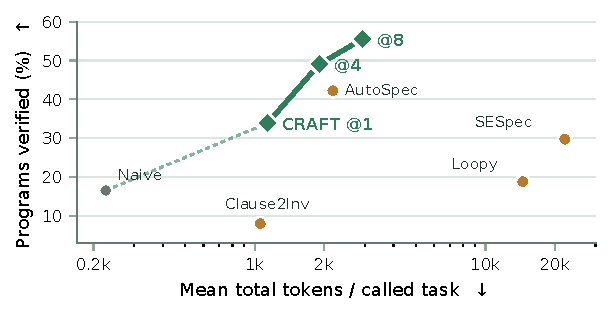
\includegraphics[width=\linewidth]{figures/tool_pareto.pdf}
\caption{GPT-5-nano accuracy--token frontier; upper-left is better.}
\label{fig:tool-pareto}
\vspace{-0.6\baselineskip}
\end{wrapfigure}
We compare \sam{} with the target-hidden pipelines of AutoSpec, SESpec,
Clause2Inv, Loopy, and Daikon~\citep{wen2024enchanting,yang2026sespec,
cao2025clause2inv,kamath2023finding,daikon}.  All LLM-based systems use
GPT-5-nano with reasoning disabled, all outputs face the same untouched
Frama-C/WP judge, and unsupported inputs count as failures among all 832
programs.  Figure~\ref{fig:tool-pareto} compares verification rate against
mean total tokens under each system's native orchestration.  All three
\sam{} budgets lie on the model-matched Pareto frontier: compose@4 verifies
49.04\% with fewer tokens than AutoSpec, the strongest external baseline in
this reasoning-disabled comparison (42.19\%), while compose@8 reaches
55.53\%.

We compare systems end to end without matching calls or token
budgets.  Appendix~\ref{app:complete-results} reports accuracy by category,
token use, runtime, and reasoning effort.  The benefit also holds for three
additional API models (Table~\ref{tab:cross-model-main}).

\begin{insightbox}
\textbf{Finding.}
Under target hiding, orchestration efficiency matters alongside proposal
strength.  CRAFT turns independent responses into reusable clauses: all three
tested budgets lie on the model-matched Pareto frontier, and compose@4
simultaneously beats the strongest external baseline in verification rate and
mean tokens.
\end{insightbox}

% ---------------------------------------------------------------------------
\subsection{RQ4: How Does RL Reshape Compositional Exploration Before and After SFT?}
\label{sec:exp:rl}

Prior work suggests that RLVR can reallocate probability toward behaviors
already available to the base model rather than create fundamentally new
reasoning patterns~\citep{yue2025rlcapacity}.  We test this at the level of
compositional utility using matched Bare--RL and SFT--SFT+RL Qwen3-8B pairs.

With Full decompose credit, RL from Bare raises compose@1 from
37.86\% to 57.93\% (+20.07 points), whereas compose@32 rises from
57.81\% to 73.20\% (+15.39 points).  After SFT, RL raises compose@1
from 63.90\% to 69.23\% (+5.33 points), while compose@32 changes from
77.90\% to 78.37\% (+0.47 points; Table~\ref{tab:reward-ablation}).
These results are consistent with RL primarily increasing the sampling
probability of existing composable clauses rather than creating new reasoning
patterns, especially after SFT initialization.  After SFT, the substantial
compose@1 gain alongside the small compose@32 gain suggests that useful
clauses become available earlier in sampling.  From Bare, the larger gain
at compose@32 is also compatible with making previously rare capabilities
more accessible; the finite-budget curves alone do not distinguish this
explanation from the emergence of new reasoning patterns.

Meanwhile, after SFT, pass@1 falls from 41.93\% to 30.78\%.
This is compatible with rewarding useful surviving clauses rather than
requiring their entire response to succeed independently.

\begin{insightbox}
\textbf{Finding.}
RL makes useful clauses available with fewer samples: its composition gains
are larger at one response than at 32, both before and after SFT.
\end{insightbox}

% ---------------------------------------------------------------------------
\subsection{RQ5: How Should Credit Be Assigned for Compositional Inference?}
\label{sec:exp:ablations}

Because targets remain hidden during RL, we use negative coverage of the
pooled survivors as a target-independent surrogate.  From the same Qwen3-8B
Bare initialization, Binary and Whole-rollout use response-level credit,
Full decompose credit preserves credit for surviving \(V_i\)
(Equation~\eqref{eq:generation-reward}); all other settings are fixed.

\begin{figure}[H]
\centering

\includegraphics[width=\textwidth]{figures/reward_ablation.pdf}
\caption{Qwen3-8B reward ablations from the Bare initialization.
  Whole-response credit reduces composition; clause credit recovers
  it.  The matched SFT-initialized controls, where Binary collapses the
  strong SFT composition curve, are in Table~\ref{tab:reward-ablation}.}
\label{fig:reward-ablation}
\end{figure}

Binary reaches only 23.32\% compose@32, below Bare's 57.81\%, showing
that rewarding inductive validity alone is insufficient to preserve
compositional performance in this setting.  Whole-rollout adds a strength
signal but retains the whole-response correctness gate; comparing it with
Full decompose credit isolates the effect of that gate.

Whole-rollout credit raises pass@1 from 6.43\% to 16.67\% yet reduces
compose@32 from 57.81\% to 22.72\%.  This exposes a tension between
single-response correctness and exploration breadth.  Its all-or-nothing
gate withholds credit from every useful surviving clause whenever any clause
in the response is rejected.  The observed composition loss is consistent
with suppressing useful partial candidates that pooled inference can exploit.
Full decompose credit removes the gate and credits
each response for the coverage of its surviving \(V_i\).  Relative to
Whole-rollout, it raises compose@1 from 18.87\% to 57.93\% and compose@32 from
22.72\% to 73.20\%, surpassing Bare by 20.07 and 15.39 points, respectively.
The available SFT-initialized and cross-backbone controls are reported in
Table~\ref{tab:reward-ablation}.

\begin{insightbox}
\textbf{Finding.}
Training credit should reflect the clauses retained by compositional
inference.  Full decompose credit preserves useful contributions lost
under Whole-rollout's all-or-nothing reward.
\end{insightbox}
